%%%%%%%%%%%%%%%%%%%%%%%%%%%%%%%%%%%%%%%%%%%%%%%%%%%%%%%%%%%%
%%
%%  BIO-SPECTRAL IMAGING REVIEW
%%	Onur Ozcelik, Sabri Bolkar
%%
%%	Summer 2015
%%%%%%%%%%%%%%%%%%%%%%%%%%%%%%%%%%%%%%%%%%%%%%%%%%%%%%%%%%%%


%%%%%%%%%% STARTING %%%%%%%%%%%%%%%%%%%%%%%%%


\documentclass[a4paper]{article}


%%%%%%%%%% PACKAGES USED %%%%%%%%%%%%%%%%%%%%

    \usepackage[english]{babel}
    \usepackage[utf8x]{inputenc}
    
    % package for including graphics with figure-environment
    \usepackage{graphicx}
    \usepackage{hyperref}
    \usepackage{mathtools}
    % colors for hyperlinks
    % colored borders (false) colored text (true)
 \hypersetup{colorlinks=true,citecolor=black,filecolor=black,linkcolor=black,urlcolor=black}

    % package for bibliography .... BIBTEX
  %  \usepackage[authoryear,round]{natbib}

    % package for page header
    \usepackage[automark]{scrpage2}
    \pagestyle{scrheadings}
    \ihead[]{Bio-Spectral Imaging: A Review} %%%%% Head writings
    \ohead[]{\date}                 %%% date ?????????
    \cfoot[]{\pagemark} 
    \setheadsepline[122mm]{0.3mm}
	
    
    \usepackage[nottoc,numbib]{tocbibind} %%%% references appear in contents 
%%%%%%%% BODY STARTS %%%%%%%%%%%%%%%%%%%%%%%

    \begin{document}
        \title{
        \begin{figure}[!ht]
            \flushleft
                
\includegraphics[width=1\textwidth]{metu_logo.jpg}
        \end{figure}
        \vspace{1cm}
        \Huge Bio-Spectral Imaging: A Review
        }

        \vspace{1cm}

        % if you are the only author, you might use the following
        % \author{Name of student}	

        % Insert here your name and correct mail address
        \author{\Large \href{mailto:first.student@smail.fh-koeln.de}{
        Onur {\"O}z{\c{c}}elik} \and \Large \href{mailto:second.student@smail.fh-koeln.de}{Sabri Bolkar} %%%% ADD MAILS 
        \vspace{1cm}}

        % name of the course and module
        \date{
       %% \large Module: Modulename \\ Course: Coursename \\ 
        \vspace{0.8cm}
        \large Supervisor: Asst. 
        Prof. Sevin{\c{c}} Figen {\"O}ktem \\
        \vspace{1cm}
        \large %%% DATE ?
        }

        \maketitle
        \setlength{\parindent}{0pt}

    \vspace{2cm}


%%%%%%%%%%%%%%%%%% ABSTRACT %%%%%%%%%%%%%%%%

    \begin{abstract}
	 Spectral Imaging is a promising optical technique that combines advantages of both spectroscopy and imaging in an unique way. It offers a noninvasive diagnostic method for numerous diseases especially for the ones that originates from epithelial tissues. Herein, this report gives an introductory overview of bio-spectral imaging and its main medical applications. It also briefly describes system hardware and main instruments that constitute bio-spectral imaging devices.  
    \end{abstract}

%%%%%%%%%%%%%%%%%%%%% INTRODUCTION %%%%%%%%%

        \newpage
        \tableofcontents
        \vspace{3cm}
        \listoffigures
        \newpage


    \section{Introduction} % (fold)
    \label{sec:Introduction}
	$\hspace{5mm}$ Spectral Imaging is a very special imaging method which extracts characteristic spectral information of elements covering the imagined area. Unlike other optical imaging methods (e.g., optical coherence tomography, optical diffuse tomography) which are monochromatic in their nature, spectral imaging utilizes different band gaps of electromagnetic spectrum and combines them to acquire all the available chemical fingerprints of ingredients as much as the current technology allows. Because of this reason, data in SI systems is stored as 3D cubes (x, y, $\lambda$) rather than mere 2d monochromatic images. As put by Qin, It can also be described as a very special multidimensional spectroscopy device that applies spectroscopic measurement for each point in imagined area: "If conventional imaging tries to answer the question \emph{where} and conventional spectroscopy tries to answer the question \emph{what}, then hyperspectral imaging tries to answer the question \emph{where} is \emph{what}" \cite{sifir}.  
    \medskip
    \begin{figure}[h]
		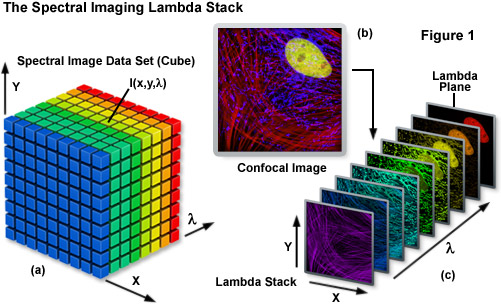
\includegraphics[width=0.5\textwidth]{3dcube.jpg}
			\centering
         \caption{3d Data Cube (Source: Zeiss-Campus)}
	\end{figure}
    	
     $\hspace{5mm}$ In the scientific literature, spectral imaging modality (i.e., imaging spectroscopy, once it was called) is divided into four main groups according to amount of spectral bands scanned. Names of research groups also indicate number of wavelengths utilized (i.e., Multispectral, hyperspectral and ultraspectral imaging). The term multispectral imaging is used to express the method that utilize only a few wavelengths to extract information. Hyperspectral imaging, Unlike multispectral imaging, includes hundreds of overlapping contagious bands, and ensures no spectral bands are skipped. And, ultraspectral imaging is much more advanced technique that includes thousands of contagious bands.   

\medskip
    $\hspace{5mm}$If conventional color cameras are to be compared with spectral imaging cameras, huge differences can be observed. Traditional cameras usually uses a single imaging chip which consists of color filters covering every pixel of a sensor. Each pixel of the sensor can detect only one of the three primary colors. Therefore, three pixels are required to detect the color of the area. Color cameras record three spectral bands simultaneously to obtain the color image and represent the image with three parameters: Red-Green-Blue, or RGB (figure 2). This cameras emulates the human vision and easy to interpret. However, similar to human vision, they have limitations. They misses spectral information outside of the three bands which is important for identifying a material. Therefore, color imaging systems cannot distinguish between different materials with the same color. This significantly limits diagnostic capabilities of color cameras and unveils the need for a more advanced system. This problem can be pointed as the main motivation behind spectral imaging architecture. Since, they obtain images at many wavelengths which are not recognizable by human vision and carries unique information about many materials which are not available with RGB cameras.
    \medskip
    \begin{figure}[h]
		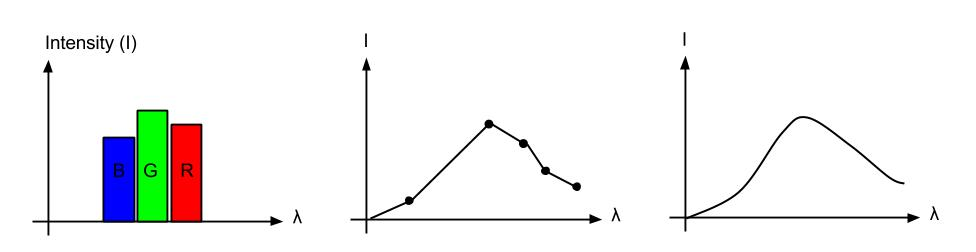
\includegraphics[width=0.8\textwidth]{rgb.jpg}
			\centering
         \caption{Spectral Scanning - comparison of RGB, multispectral and hyperspectral imaging methods}
	\end{figure}
    
    \section{Origins of Bio-Spectral Imaging}
    \label{sub:origins_of_Bio-Spectral_Imaging}
    
    $\hspace{5mm}$ The idea to use several spectral signatures of elements dates back to 1970's when a detailed analysis was needed for remote sensing applications (i.e., NASA  Landsat-1 in 1972 transferred intense spectral data). As put by Alexander Goetz, who is the main figure behind this miraculous method, it was the enormous noisy data that led this great invention: "No single material requires hundreds of spectral bands spread over several octaves of the electromagnetic spectrum to be identified uniquely. However, when mixed with many other materials on the Earth's surface and viewed through a hostile and changing atmosphere, there is security in numbers." But, at that time the problem was the limited technology to analyze collected data since improvements in the field was highly stick to the advances in computational power. It was 90's when spectral imaging technique fully exploited \cite{bir}. A timeline for spectral imaging airborne and satellite cameras can be viewed in figure 3. 
    \medskip
    \begin{figure}[h]
		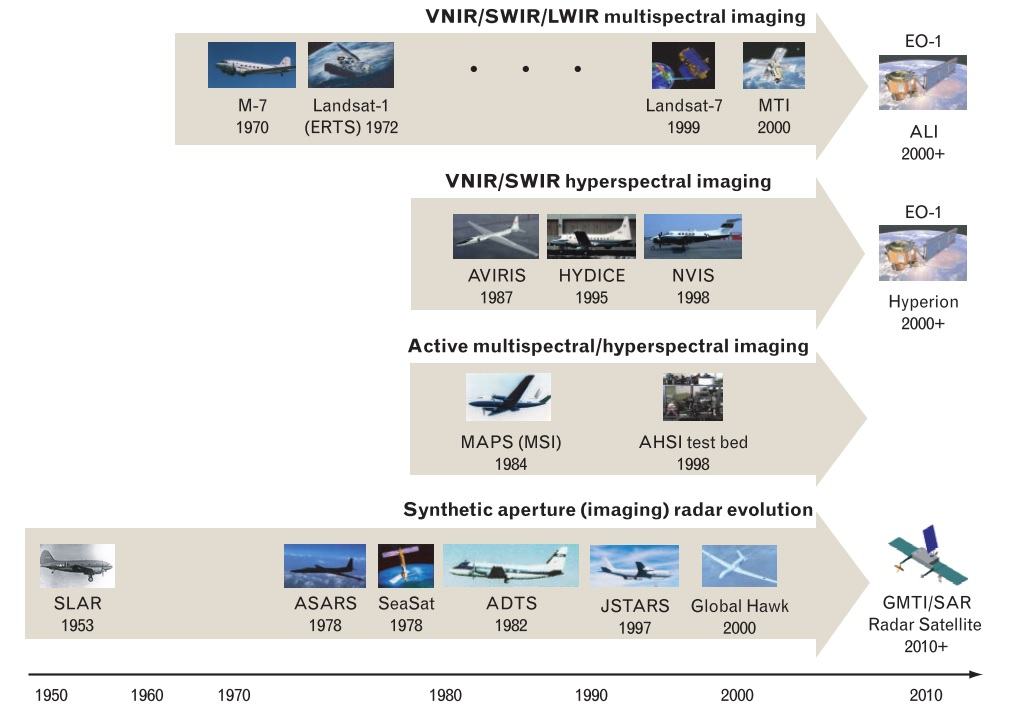
\includegraphics[width=0.9\textwidth]{timeline.jpg}
			\centering
         \caption{Timeline of three different categories of spectral imaging, along with synthetic aperture radar (SAR) imaging \cite{iki}}
	\end{figure} 
    
    $\hspace{5mm}$ Before 90's, remote sensing SI devices were not suitable for laboratory use and for bio-applications because of their high cost, large size and complexity. However, after late 80's, advances in computational power and increase in availability of low cost sensors (e.g., CCD detectors) enabled biomedical implementation of spectral imaging technique \cite{uc}. One of the early successful application of the technique came with the name SpectraCube\texttrademark 1000, developed in 1994 by a team from Bar Ilan University and Spectral-Diagnostics\texttrademark \cite{dort}. It stands as the first successful implementation of the idea. Although the system's spatial resolution was quite low (just 170$\times$170), it was able to observe subcellular characteristics of cells (i.e., visualization of chromatin packing, determination of porphyrin level and distribution of cytoplasmic organelles). Later, spectral imaging had become more common in biomedical society. Institutions started to create their own spectral imaging devices for many other diagnosis and research purposes. More detailed analysis of these different spectral imaging systems will be given in the following sections of the article. 



%%%%%%%%%%%%%%%%%  HARDWARE OVERVIEW %%%%%%%%%%%%

	\section{Hardware of Bio-Spectral Imaging Devices: Instruments}
    \label{sec:Hardware_of_Bio-Spectral_Imaging_Devices}
    \hspace{5mm} A typical bio-spectral imaging system consists of five main instruments: \emph{Light source} to create information carrier signal interacting with matter, \emph{wavelength dispersion device} to read spectral information from white light, \emph{imaging detector} such as CCD and CMOS area detectors, \emph{data analysis element} (e.g., computer) and \emph{calibration module} for spectral and spatial calibration (figure 4), for most of the modern systems calibration module and other peripherals are embedded to the main computer to ease the control of the information flow.
    \medskip
    \begin{figure}[h]
		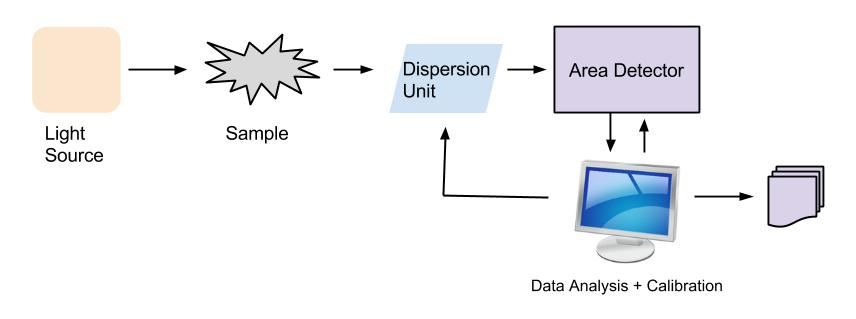
\includegraphics[width=0.9\textwidth]{system.jpg}
			\centering
         \caption{SI system overview}
	\end{figure}
    
    \hspace{5mm} The core part of the bio-spectral imaging architecture is the light source. Unlike its predecessor remote sensing hyperspectral imaging systems, bio-spectral imaging devices uses active light to acquire knowledge from the sample (i.e., if natural light sources are used, the system is called passive imaging system as in the case of most of the remote sensing applications). The main aim of the light source is to create the means of interaction with material to be scanned. Instruments utilized as imaging light sources are: Halogen lamps, light emitting diodes (LED), lasers. There exist also another type of sources which are called tunable sources. Systems using this approach are rather different with respect to system architecture. They reverse the order and place dispersion element before sample, so that matter interacting light become dispersed \cite{sifir}.
    
    \medskip
    \hspace{5mm} The system element dispersing broadband light to its monochromatic constituents is called wavelength dispersion device. Because imaging sensors are physically color blind (i.e., they are only sensible to specific photon energy levels, only specific monochromatic light), broadband light has to be dispersed to be able to measure intensity level for each wavelength. Main instruments utilized for this purpose are: Interferometers (e.g., Michelson Interferometer, Sagnac Interferometer), imaging spectrographs, filter wheels, Acousto-optic tunable filters (AOTF), liquid crystal tunable filters (LCTF) and specialized dispersion devices used in snapshot imaging methods \cite{bes} \cite{sifir}.
    
    \medskip
    \hspace{5mm} Third major component of bio-spectral imaging systems are area detectors. After dispersion of spectral information carrier light, components of light are directed to CCD and CMOS image sensors. They differ from traditional spectroscopy detectors and are able image an configured area (i.e., in spectroscopy, point detectors are used).
						
										
%%%%%%%%%%%%%%%%%%%%%%%%%%%%%%%%%%%%%

 \section{Fundamentals of Bio-Spectral Imaging} % (fold)
    \label{sec:Fundamentals_of_Bio-Spectral_Imaging}
    \hspace{5mm} Interaction of light with targeted tissue is the most important research topic in bio-spectral imaging. As the information carrying medium, light should be able to penetrate the tissue to reach the target, interrogate with cells and it also should be recaptured by sensors to acquire related information \cite{bes.1}. In each of these processes, there exist deep bio-physical interaction models and theories which are above the scope of this article. But, it is essential to delve into fundamental ideas about tissue optics and discussions why spectral imaging is a great choice of diagnosis technique.  
    
    \medskip
     \hspace{5mm} There exist four main interactions of light photons with matter: Absorption, refraction, scattering and transmission, all of which occur at atomic scale and alter the state of light according to characteristic differences of interacted cells. In addition to these fundamental processes, there are also some additional optical parameters that can be used to characterize tissues such as anisotropy (i.e., directional dependency of interacting materials) and reduced scattering \cite{bes.1}. The first process light undergoes is absorption, the later processes are possible when energy level of light photon is not suitable for absorption, and photon escapes from first danger. After interacting with matter (e.g., scattered, refracted) photon's energy level is lowered and probability of absorption increases. In all of these interactions light carries embedded fingerprints of the chemical structure even in absorption. Since, after absorption increase in the energy of the material may lead to re-emission or heat generation (even chemical reactions) that makes materials observable \cite{bes.2}.
       \medskip
    \begin{figure}[h]
		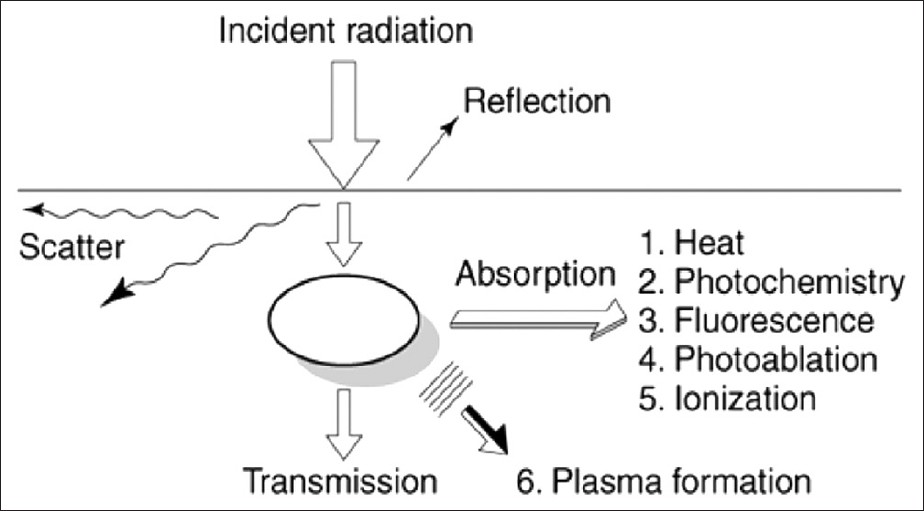
\includegraphics[width=0.7\textwidth]{light_tissue.jpg}
			\centering
         \caption{Light Tissue Interaction \cite{onbir}}
	\end{figure}
     
    \hspace{5mm} Most tissues in human body are heterogeneous; therefore, spatial variations can be seen in their optical properties. Because of spatial variations, most of light photons are scattered within human tissues \cite{alti}. The penetration depth of light into tissues depends on how strongly light is absorbed by these tissues. Most tissues cannot absorb enough light to permit it to penetrate significantly in the spectral range from 600 to 1300 nanometer, known as diagnostic window. Within this window, the propagating light becomes diffuse because scattering is dominant over absorption \cite{alti} \cite{yedi}. In tissues, absorption is a function of molecular composition, whose changes at specific wavelengths could provide a spectral fingerprint of the molecule for diagnosis \cite{alti} \cite{sekiz}. Light absorbed by tissues could be radiated as fluorescence. Ultraviolet and visible light usually excite the molecules of the tissues and causes fluorescence emission. Different fluorescence emission spectra could be observed in different cells which are in different disease states. Therefore, fluorescence imaging can be used to inspect tissues for medical diagnosis \cite{yedi}.


%%%%%%%%%%%%%%%%%%%%%%%%%%%%%%%%%%

 \section{Classification of Imaging Systems} % (fold)
    \label{sec:Classification_of_Imaging_Systems}
   

  

    \subsection{According to Spatial Scanning Methods} % (fold)
    \label{sub:According_to_Spatial_Scanning_Methods}
    
    \hspace{5mm} Monochrome sensors used in spectral imaging systems can capture only two of three spectral dimensions (x, y, $\lambda$) of the spectral cube at a time. Spatial or spectral scanning methods are used to capture the third dimension \cite{dokuz}. The whiskbroom, pushbroom, staring and snapshot (single exposure) methods are commonly used in bio-spectral imaging applications \cite{bes}.
		
     \medskip   
	 \hspace{5mm} In Whiskbroom method, spectrum ($\lambda$) of a single point is obtained by sensor arrays at a time and the point is scanned along two spatial dimensions (x and y). In Pushbroom method, one spatial dimension (x) and spectrum ($\lambda$) is obtained with a 2D detector array and the other spatial dimension (y) is captured with line scanning. Whiskbroom and Pushbroom methods require a lot time to acquire spectral cube because they do spatial scanning and intense data processing is required. Another disadvantage of these methods is that they usually require complex hardware configurations. In Whiskbroom and Pushbroom methods, light is divided by a dispersive element (prism or grating), which makes them efficient and low-cost \cite{bes}.

	 \medskip   
	 \hspace{5mm} Pushbroom method is suitable for searching an object with specific spectra, because line-scan provides the entire spectrum of each pixel in real time. With Pushbroom method, the entire spectral cube does not have to be collected. For a known spectrum, a classified image can be assembled by identifying the spectrum in each spectral line scan \cite{on}

	\medskip   
	 \hspace{5mm} In Staring method, full spatial image (x and y) is obtained at once with a 2D sensor array while the spectrum ($\lambda$) is scanned. Instead of the dispersive element used in Whiskbroom and Pushbroom methods, tunable filters are used in this method and because of that, the spectral cube can be acquired in a simpler way without any relative motion of the scene and the imager \cite{oniki}. In staring method, the number of spectral bands scanned can be determined by the user and a dynamic range can be maintained \cite{bes}. Also, in clinical applications, staring spectral imagining devices become more suitable when imagined area is exposed to wide field (broadband) illumination \cite{dokuz}.
     
	\medskip   
	 \hspace{5mm} In Snapshot method, the spatial image (x and y) and the spectrum ($\lambda$) is obtained in a single exposure. One of the advantages of the snapshot method is that spectral image can be captured faster than other methods. Therefore, it can be used in studies in endoscopy detection, fluorescent probes analysis and retinal oxygen saturation measurement. Another advantage of this method is high reliability and robustness since snapshot imagers has no moving parts. It also provide high throughput because there are no multiplex losses. The disadvantage of the snapshot method is low spatial resolution because the size of the spectral cube depends on the size of the CCD sensor used in the imager \cite{alti}.


%%%%%%%%%%%%%%%%%%%%%%%%%%%%%%%%%%%%%%%%%%%%%%%%%%%%%%%%%%%%%


    \subsection{According to Spectroscopic Measurement Types} % (fold)
    \label{sub:According_to_Spectroscopic_Measurement_Types}
			
            \medskip
            \hspace{5mm}The other type of classification is based on measurement methods. To collect spectral data from different type of tissues, several techniques have been developed. All of the methods will be discussed have various advantages over others, especially when analyzing different tissues having unique optical characteristics. Therefore, considerations related with optical properties of tissues are crucial when choosing the optimal imaging modality. 
            
            \medskip
           \subsubsection{Near-infrared Spectral Imaging (NIR-SI)}
           \hspace{5mm} NIR spectroscopy has already been used in some applications such as measurement hemoglobin concentration and blood oxygen saturation \cite{onuc}. Near-infrared imaging can be used as a complementary method for tissue characterization and diagnosis of cancer because of its ability to distinguishing normal tissue from diseased tissue. NIR light between 700 and 900 nm is mostly scattered in tissues and it can reach deep tissues. Unlike the other imaging methods such as X-ray and MRI, extra harmful radiation or radioactive materials are not used in NIR imaging \cite{ondort}. 

           \subsubsection{Reflectance SI}
           \hspace{5mm} Diseased tissues interact with light in some ways like elastic scattering and absorption. When light interacts with a diseased tissue, the effect of the disease on the tissue causes some changes in the patterns in the light. These changes can be seen on the light reflected from the tissue. There are several studies investigating the applications of reflectance spectroscopy for tissues in cervix, breast, oral cavity, lungs, esophagus and gastrointestinal tract. There are also applications of reflectance spectroscopy for brain tumors, ovarian cancer, bladder cancer and skin cancer \cite{onbes}. 
          
            \subsubsection{Fluorescence SI}
            \hspace{5mm} Fluorescence is used in a wide range of applications such as fluorescence microscopy, DNA sequencing, flow cytometry and fluorescence-based immunoassays. In biomedical applications, fluorescence spectroscopy has been being investigated for applications such as characterizing cardiac tissue, analyzing blood and early detection of cancer, particularly those in the cervix, oral cavity, breast, brain, skin, esophagus and bronchus \cite{onalti}.

            \subsubsection{Light Scattering SI}
            \hspace{5mm} Light scattering spectroscopy (LSS) allows investigating the structure of epithelial cells without removing them. With the use of LSS, Images of some histological properties (e.g., nuclear enlargement, pleomorphism and increased chromatin content) can be obtained. LSS imaging shows promising results for investigation of nuclear changes resulting from cancer and other diseases, particularly cancer in cervix and oral cavity \cite{onalti.1}. Light scattering spectroscopy also shows promise for the precise classification of invisible dysplasia in real time \cite{onalti.2}.

            \subsubsection{Raman Scattering SI}
            \hspace{5mm} Raman spectroscopy can provide information about chemical and molecular properties of tissues without destructive effects and external contrast-enhancing substances. Most of the reported studies about Raman spectroscopy examined its applications in skin, although there are studies investigating its  applications in bone, brain, gastrointestinal tract, artery, breast, urinary tract, uterus, lung, and eye \cite{onalti.3}. Since it consists of a lot of components (e.g., lasers, filters, microscope objectives), Raman spectroscopy is compatible with other methods of biomedical optics such as confocal laser-scanning, optical coherence tomography and angularly resolved elastic scattering \cite{onalti.4}.


     
    %%%%%%%%%%%%%%%%%%%%%%%%%%%%%%%%%%%%%%%%%%%%%%%%%
    
    
    
    
    
%%%%%%%%%%%%%%%%%%%%%% 


\section{Spectral Imaging Data Analysis} % (fold)
    \label{sec:Spectral_Imaging_Data_Analysis}
    
    \hspace{5mm} It can be stated that diagnosis process and medical treatment cannot be possible without processing of acquired spectral data. Complexity and noisiness of raw data makes it cumbersome  to comprehend even for expert physicians. Therefore, to extract relevant feature, data is processed. General procedure for processing can be viewed in figure 6.
    
    \begin{figure}[h]
		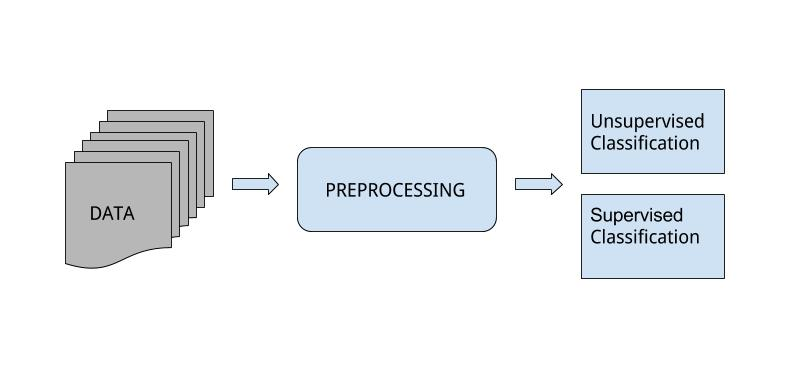
\includegraphics[width=0.7\textwidth]{dataAnaly.jpg}
			\centering
         \caption{Data Processing Steps}
	\end{figure}

	\subsection{Preprocessing}
    
    \hspace{5mm} The first step in data processing is preprocessing. As the name implies preprocessing is preparation step before real analysis is done. The data acquired by SI devices include thousands of pixels and wavelengths. Processing of high dimensional data is harder and inefficient (i.e., classification algorithms check unneeded data), therefore various preprocessing methods have been developed by engineers. In addition to its main aim easing the way to extract features, preprocessing also serves for another purpose that is decreasing so-called curse of dimensionality \cite{dokuz}.
    
    \medskip
    \hspace{5mm} Curse of dimensionality is accepted as one of the most important issues in machine learning field. The term was coined in 1961 by Richard Bellman while he was working of dynamic optimization \cite{onyedi}. This infamous term has been popularized because of its counter-intuitive results. Increasing data dimension may lead to expectation of more accurate results, but in contrast it is the high dimensional data itself scrambles the classifier. This strange outcome is the main reason for necessity of a preprocessor to lower data dimension.
It should be stated that preprocessing algorithms are optimized not to lose any information while decreasing dimension of data \cite{onsekiz}. Principal component analysis is one of the main methods for preprocessing applications, there exists also an advanced form of PCA called independent component analysis (ICA) which can also be used as preprocessor, but it's mainly used as classifier especially for brain signal analysis. A detailed and simplified information about PCA can be found in Shlen's famous tutorial \cite{ondokuz}.  

	
    \subsection{Classification}
    
    \hspace{5mm} After removal of redundancy in data by preprocessing algorithms, remaining data space is fed to classifier. Classifier is the main part in machine learning systems where data is separated according to their feature components each having unique characteristics. There are various ways to do that job, but classifiers are generally divided into two groups: Supervised Clustering and Unsupervised Clustering. 
    
     \begin{figure}[h]
		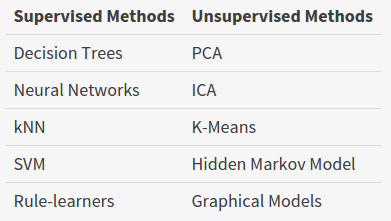
\includegraphics[width=0.6\textwidth]{Class.png}
			\centering
         \caption{Main classifier algorithms}
	\end{figure}
    
    \newpage
    
    \hspace{5mm} Both supervised and unsupervised methods depends upon statistical resemblance mapping in which data points are selected and classified to maximize (or minimize) targeted statistical parameter. Discussion related with classification algorithms is out of the scope of this paper because of intense research done on machine learning algorithms. But, some of the most used algorithms can be viewed in Figure 7.
    
   
    
    \subsection{Spectral Unmixing}
    
    \hspace{5mm} Distribution of materials in spectral data cube is generally heterogeneous; and a single pixel does not contain just one type of material. Therefore, there is a need for sub-pixel analysis. The method to extract sub-pixel features is called \emph{Spectral Unmixing}. It is used to approximate material ingredients using known spectral of materials and pixel's spectra. In other words, it is in a way a sub-pixel spectral decomposer for spectral imaging systems \cite{yirmi}.
    
    
     \begin{figure}[h]
		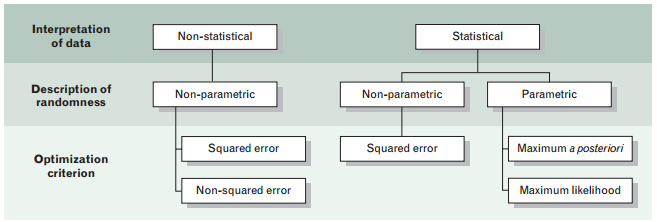
\includegraphics[width=1\textwidth]{unmix.png}
			\centering
         \caption{Taxonomy of Unmixing Algorithms \cite{yirmi}}
	\end{figure}
%%%%%%%%%%%%%%%%%%%%%%%%%%%%%%%%%%%%
	\newpage
    \section{Conclusion} % (fold)
    \label{sec:conclusion}
    
    \hspace{5mm} We have presented mainstream spectral imaging applications in medical diagnosis and treatment. The article is aimed to be an introductory text for explaining general concepts without going into too much detail. In addition to medical applications and spectral imaging methods, SI instruments, brief history of hyperspectral imaging and data analysis techniques are also discussed. We also referenced most cited and inclusive articles that fit best for beginners in the bio-spectral imaging research field, therefore further investigation can be easily done through reading sources referenced. 
    
    \medskip
    \hspace{5mm}



%%%%%%%%%%%%%%%%%%%%%%%%%%%%%%%%%%

%%	\section{Glossary}
  %%  \label{sec:Glossary}


%%%%%%%%%%%%%%%%%%%%%%%%%%%%%%%%%%%%


 
%%%%%%%%%%%%%%%%%%%%%%%%%%%%%%%%%%%%%%%%%% REFERANCES 
   

   %% \bibliographystyle{natdin}  .... BIBTEX
     %%   \bibliography{references} % expects file "references.bib"

\begin{thebibliography}{9}

\bibitem{sifir} Qin, J. (2010). Hyperspectral Imaging Instruments. Da-Wen, S.(ed.) in \emph{Hyperspectral Imaging for Food Quality Analysis and Control}. Elsevier. http://doi.org/10.1016/B978-0-12-374753-2.10005-X

\bibitem{bir} Goetz, A. F. H. (2009). Three decades of hyperspectral remote sensing of the Earth: A personal view. \emph{Remote Sensing of Environment}, 113(SUPPL. 1), 5–16. http://doi.org/10.1016/j.rse.2007.12.014

\bibitem{iki} Shaw, G. Burke, H. (2003). Spectral Imaging for Remote Sensing. \emph{Lincoln Lab. Journal}, 14(1). 

\bibitem{uc} Garini, Y., Katzir, N., Cabib, D., Buckwald, R. a, Soenksen, D. G., Malik, Z. (1996). Spectral Bio-Imaging. \emph{Fluorescence Imaging Spectroscopy and Microscopy.}  

\bibitem{dort} Zvi Malik ; Dario Cabib ; Robert A. Buckwald ; Yuval Garini and Dirk G. Soenksen "Novel spectral imaging system combining spectroscopy with imaging applications for biology", Proc. SPIE 2329, \emph{Optical and Imaging Techniques in Biomedicine}, 180 (February 1, 1995)

\bibitem{bes} Li, Q., He, X., Wang, Y., Liu, H., Xu, D., and Guo, F. (2013). Review of spectral imaging technology in biomedical engineering: achievements and challenges. \emph{Journal of Biomedical Optics}, 18(10), 100901. http://doi.org/10.1117/1.JBO.18.10.100901

\bibitem{bes.1} Jacques, S. L. (2013). Optical Properties of Biological Tissues: A Review. \emph{Physics in Medicine and Biology}, 58(11), R37–61. 

\bibitem{bes.2} Walsh, J. (2011).Basic Interactions of Light with Tissue. Welch, A. J.,  Van Gemert, M. J. C.(ed.) In \emph{Optical-thermal response of laser-irradiated tissue}, 1–958. http://doi.org/10.1007/978-90-481-8831-4

\bibitem{alti} Joel, M. (2003). Optical Properties of Tissues. Vo-Dinh (ed.) In \emph{Biomedical Photonics Handbook}. CRC Press. 

\bibitem{yedi} Lu, G., and Fei, B. (2014). Medical hyperspectral imaging: a review. \emph{Journal of Biomedical Optics}, 19(1), 10901. 

\bibitem{sekiz} Zhang, Y., Chen, Y., Yu, Y., Xue, X., Tuchin, V. V, and Zhu, D. (2013). Visible and near-infrared spectroscopy for distinguishing malignant tumor tissue from benign tumor and normal breast tissues in vitro. \emph{Journal of Biomedical Optics}, 18(7), 077003. 

\bibitem{dokuz} Balas, C. et al. (2011). Multi/Hyper-spectral Imaging. Boas, D. A. et al (ed.) in \emph{Handbook of biomedical optics}. Boca Raton : CRC Press, c2011.

\bibitem{on} Bearman, G. and Levenson, L.(2003). Biological Imaging Spectroscopy. Vo-Dinh (ed.) In \emph{Biomedical Photonics Handbook}. CRC Press. 

\bibitem{onbir} Elavarasu S, Naveen D, Thangavelu A. Lasers in periodontics. J Pharm Bioall Sci [serial online] 2012 [cited 2015 Aug 30];4, Suppl S2:260-3. Available from: http://www.jpbsonline.org/text.asp?2012/4/6/260/100245

\bibitem{oniki} N. Gupta, “Development of staring hyperspectral imagers,” in 2011 IEEE Applied Imagery Pattern Recognition Workshop, Washington, DC, pp. 1–8, Institute of Electrical and Electronics Engineers Inc. (2011).

\bibitem{onuc} Yu, G. et al. (2011). Near-Infrared Diffuse Correlation Spectroscopy for Assessment of Tissue Blood Flow. Boas, D. A. et al (ed.) in \emph{Handbook of biomedical optics}. Boca Raton : CRC Press, c2011.

\bibitem{ondort} Erickson, S. J., \& Godavarty, A. (2009). Hand-held based near-infrared optical imaging devices: A review. Medical Engineering and Physics, 31(5), 495–509. http://doi.org/10.1016/j.medengphy.2008.10.004

\bibitem{onbes} McGee, S. et al. (2011). Reflectance Spectroscopy. Boas, D. A. et al (ed.) in \emph{Handbook of biomedical optics}. Boca Raton : CRC Press, c2011.

\bibitem{onalti} Roblyer, D. et al. (2011). Fluorescence Spectroscopy. Boas, D. A. et al (ed.) in \emph{Handbook of biomedical optics}. Boca Raton : CRC Press, c2011.

\bibitem{onalti.1} Gurjar, R.S., Backman, V., Perelman, L.T., Georgakoudi, I., Badizadegan, K.,
Itzkan, I., Dasari, R.R., Feld, M.S. (2001). Imaging human epithelial
properties with polarized light-scattering spectroscopy. \emph{Nature Med.}, 7(11),
1245–1248.

\bibitem{onalti.2} Qiu, L. et al. (2011). Light Scattering Spectroscopy. Boas, D. A. et al (ed.) in \emph{Handbook of biomedical optics}. Boca Raton : CRC Press, c2011.

\bibitem{onalti.3} Krafft, C., \& Sergo, V. (2006). Biomedical applications of Raman and infrared spectroscopy to diagnose tissues. \emph{Spectroscopy}, 20(5-6), 195–218.

\bibitem{onalti.4} Berger, A.J. (2011). Raman, SERS, and FTIR Spectroscopy. Boas, D. A. et al (ed.) in \emph{Handbook of biomedical optics}. Boca Raton : CRC Press, c2011.

\bibitem{onyedi} Bellman, R. E (1961). \emph{Adaptive control processes: a guided tour.} Princeton University Press

\bibitem{onsekiz} Domingos, P. (2012). A few useful things to know about machine learning. Communications of the ACM, 55(10), 78. 

\bibitem{ondokuz} Shlens, J. (2014). A Tutorial on Principal Component Analysis. Retrieved from http://arxiv.org/abs/1404.1100

\bibitem{yirmi} Keshava, N. (2003). A Survey of Spectral Unmixing Algorithms. Lincoln Laboratory Journal, 14(1), 55–78. 

\end{thebibliography}

%%%%%%%%%%%%%%%%%%%%%%%%%%%%%%%%%%%%%%%%%%


\end{document}

